


%% This is file `sample-authordraft.tex',
%% generated with the docstrip utility.
%%
%% The original source files were:
%%
%% samples.dtx  (with options: `authordraft')
%% 
%% IMPORTANT NOTICE:
%% 
%% For the copyright see the source file.
%% 
%% Any modified versions of this file must be renamed
%% with new filenames distinct from sample-authordraft.tex.
%% 
%% For distribution of the original source see the terms
%% for copying and modification in the file samples.dtx.
%% 
%% This generated file may be distributed as long as the
%% original source files, as listed above, are part of the
%% same distribution. (The sources need not necessarily be
%% in the same archive or directory.)
%%
%% The first command in your LaTeX source must be the \documentclass command.
\documentclass[sigconf]{acmart}
\usepackage{graphicx}
\usepackage{comment}
\usepackage{amsmath,amssymb} % define this before the line numbering.
\usepackage{color}
\usepackage{booktabs}
\usepackage{algorithm}
\usepackage{siunitx}
\usepackage[noend]{algpseudocode}
\usepackage{wrapfig,lipsum,booktabs}
\usepackage{enumerate}   
% INITIAL SUBMISSION - The following two lines are NOT commented
% CAMERA READY - Comment OUT the following two lines
\usepackage[width=122mm,left=12mm,paperwidth=146mm,height=193mm,top=12mm,paperheight=217mm]{geometry}

%%%%%%%%%%%%%%%%%%%%%%%%%%%%%%%%%%%%% my usage
\usepackage{helvet} % DO NOT CHANGE THIS
\usepackage{courier}  % DO NOT CHANGE THIS
\usepackage[square]{natbib}
\usepackage[utf8]{inputenc} % allow utf-8 input
\usepackage[T1]{fontenc}    % use 8-bit T1 fonts
\usepackage{hyperref}

\usepackage{booktabs}       % professional-quality tables
\usepackage{amsfonts}       % blackboard math symbols
\usepackage{nicefrac}       % closed symbols for 1/2, etc.
\usepackage{microtype}      % microtypography


\usepackage{epsfig}
\usepackage{amsmath}
\usepackage{amssymb}
\usepackage{adjustbox}

% Include other packages here, before hyperref.
%\usepackage{algorithm}
%\usepackage{algorithmic}
\usepackage{amsthm}  
\usepackage{wasysym}
\usepackage[ruled,vlined,algo2e]{algorithm2e}
\providecommand{\SetAlgoLined}{\SetLine}
\usepackage{color}
\usepackage{dsfont}	
\usepackage{wrapfig}
\usepackage{footnote}
\usepackage{epstopdf}
 \usepackage{enumitem}
% \usepackage{subfigure}
\usepackage{caption}
\usepackage{subcaption}
% \usepackage{subfigure}
\usepackage{comment}
\usepackage{multirow}

\def\resp{\emph{resp. }}
\def\eg{\emph{e.g., }}
\def\ie{\emph{i.e., }}
\def\cf{\emph{c.f. }}
\def\etc{\emph{etc. }} 
\def\vs{\emph{vs. }}
\def\wrt{\emph{w.r.t. }}
\def\etal{\emph{et al. }}
\def\cac{{\sc corpus }}
\def\lidar{LiDAR}
\def\lodo{LodoNet}

\usepackage{pifont}% http://ctan.org/pkg/pifont
\newcommand{\cmark}{\ding{51}}%
\newcommand{\xmark}{\ding{55}}%

\DeclareMathOperator*{\argmin}{arg\,min}
\DeclareMathOperator*{\argmax}{arg\,max}
\usepackage{mathtools}
\DeclarePairedDelimiter\ceil{\lceil}{\rceil}
\DeclarePairedDelimiter\floor{\lfloor}{\rfloor}

\makeatletter
\newcommand*{\rom}[1]{\expandafter\@slowromancap\romannumeral #1@}
\makeatother
\makeatletter
\newcommand\footnoteref[1]{\protected@xdef\@thefnmark{\ref{#1}}\@footnotemark}
\makeatother
\newcommand{\bfsection}[1]{\vspace*{0.1cm}\noindent\textbf{#1.}}

\newtheorem{prop}{Proposition}
% \newtheorem{lemma}{Lemma}
\newtheorem{defi}{Definition}
\newtheorem{thm}{Theorem}
\newtheorem{cor}{Corollary}


%%
%% \BibTeX command to typeset BibTeX logo in the docs
\AtBeginDocument{%
  \providecommand\BibTeX{{%
    \normalfont B\kern-0.5em{\scshape i\kern-0.25em b}\kern-0.8em\TeX}}}

%% Rights management information.  This information is sent to you
%% when you complete the rights form.  These commands have SAMPLE
%% values in them; it is your responsibility as an author to replace
%% the commands and values with those provided to you when you
%% complete the rights form.
\setcopyright{acmcopyright}
\copyrightyear{2020}
\acmYear{2020}
\acmDOI{10.1145/3394171.3413771}

%% These commands are for a PROCEEDINGS abstract or paper.
\acmConference[Seattle '20]{Seattle '20: ACM Symposium on Multimedia}{October 12--16, 2020}{Seattle, WA}
\acmBooktitle{Seattle '20: ACM Symposium on Multimedia, October 12--16, 2020, Seattle, WA}
\acmPrice{15.00}
\acmISBN{978-1-4503-7988-5/20/10}


%%
%% Submission ID.
%% Use this when submitting an article to a sponsored event. You'll
%% receive a unique submission ID from the organizers
%% of the event, and this ID should be used as the parameter to this command.
%%\acmSubmissionID{1965}

%%
%% The majority of ACM publications use numbered citations and
%% references.  The command \citestyle{authoryear} switches to the
%% "author year" style.
%%
%% If you are preparing content for an event
%% sponsored by ACM SIGGRAPH, you must use the "author year" style of
%% citations and references.
%% Uncommenting
%% the next command will enable that style.
%%\citestyle{acmauthoryear}

%%
%% end of the preamble, start of the body of the document source.
\begin{document}

%%
%% The "title" command has an optional parameter,
%% allowing the author to define a "short title" to be used in page headers.
\title{\lodo{}: A Deep Neural Network with 2D Keypoint Matching for 3D LiDAR Odometry Estimation}

%%
%% The "author" command and its associated commands are used to define
%% the authors and their affiliations.
%% Of note is the shared affiliation of the first two authors, and the
%% "authornote" and "authornotemark" commands
%% used to denote shared contribution to the research.
\author{Ce Zheng}
% \authornotemark[1]
% \authornote{Both authors contributed equally to this research.}
\email{czheng6@uncc.edu}
\affiliation{%
  \institution{The University of North Carolina at Charlotte}
}

\author{Yecheng Lyu}
% \authornotemark[2]
% \authornote{Both authors contributed equally to this research.}
\email{ylyu@wpi.edu}
\affiliation{%
  \institution{Worcester Polytechnic Institute}
}

\author{Ming Li}
% \authornotemark[2]
% \authornote{Both authors contributed equally to this research.}
\email{mli12@wpi.edu}
\affiliation{%
  \institution{Worcester Polytechnic Institute}
}

\author{Ziming Zhang}
% \authornotemark[1]
\authornote{Corresponding author}
\email{zzhang15@wpi.edu}
\affiliation{%
  \institution{Worcester Polytechnic Institute}
}
% \author{Ben Trovato}
% \authornote{Both authors contributed equally to this research.}
% \email{trovato@corporation.com}
% \orcid{1234-5678-9012}
% \author{G.K.M. Tobin}
% \authornotemark[1]
% \email{webmaster@marysville-ohio.com}
% \affiliation{%
%   \institution{Institute for Clarity in Documentation}
%   \streetaddress{P.O. Box 1212}
%   \city{Dublin}
%   \state{Ohio}
%   \postcode{43017-6221}
% }


%%
%% By default, the full list of authors will be used in the page
%% headers. Often, this list is too long, and will overlap
%% other information printed in the page headers. This command allows
%% the author to define a more concise list
%% of authors' names for this purpose.
% \renewcommand{\shortauthors}{Trovato and Tobin, et al.}

%%
%% The abstract is a short summary of the work to be presented in the
%% article.
\begin{abstract}
Deep learning based LiDAR odometry (LO) estimation attracts increasing research interests in the field of autonomous driving and robotics. Existing works feed consecutive LiDAR frames into neural networks as point clouds and match pairs in the learned feature space. %, however, they do not satisfy the requirement in accuracy. 
%In this paper, we study the problem of how to set up an effective feature space on point clouds so that precise coordinate correspondences between two LiDAR frame can be established for odometry estimation. 
In contrast, motivated by the success of image based feature extractors, we propose to transfer the LiDAR frames to image space and reformulate the problem as image feature extraction. With the help of scale-invariant feature transform (SIFT) for feature extraction, we are able to generate matched keypoint pairs (MKPs) that can be precisely returned to the 3D space. A convolutional neural network pipeline is designed for LiDAR odometry estimation by extracted MKPs. The proposed scheme, namely \lodo{}, is then evaluated in the KITTI odometry estimation benchmark, achieving on par with or even better results than the state-of-the-art. %whose result is with in the first tier in accuracy.


\end{abstract}

%%
%%
% \begin{CCSXML}
% <ccs2012>
%  <concept>
%   <concept_id>10010520.10010553.10010562</concept_id>
%   <concept_desc>Computer systems organization~Embedded systems</concept_desc>
%   <concept_significance>500</concept_significance>
%  </concept>
%  <concept>
%   <concept_id>10010520.10010575.10010755</concept_id>
%   <concept_desc>Computer systems organization~Redundancy</concept_desc>
%   <concept_significance>300</concept_significance>
%  </concept>
%  <concept>
%   <concept_id>10010520.10010553.10010554</concept_id>
%   <concept_desc>Computer systems organization~Robotics</concept_desc>
%   <concept_significance>100</concept_significance>
%  </concept>
%  <concept>
%   <concept_id>10003033.10003083.10003095</concept_id>
%   <concept_desc>Networks~Network reliability</concept_desc>
%   <concept_significance>100</concept_significance>
%  </concept>
% </ccs2012>
% \end{CCSXML}

% \ccsdesc[500]{Computer systems organization~Embedded systems}
% \ccsdesc[300]{Computer systems organization~Redundancy}
% \ccsdesc{Computer systems organization~Robotics}
% \ccsdesc[100]{Networks~Network reliability}

%%
%% Keywords. The author(s) should pick words that accurately describe
%% the work being presented. Separate the keywords with commas.
\keywords{Vehicle localization, LiDAR processing, Deep learning}

%% A "teaser" image appears between the author and affiliation
%% information and the body of the document, and typically spans the
%% page.

%%
%% This command processes the author and affiliation and title
%% information and builds the first part of the formatted document.
\maketitle

\section{Introduction}

Odometry estimation is one of the key components in the automated driving systems and robotics. In recent years, autonomous driving has attracted significant research interest and several works have been proposed to estimate the position and orientation of the autonomous vehicles. Multiple sensors are deployed to collect relative data including monocular cameras, Inertial Measurement Units (IMU), and Light Detection and Ranging (LiDAR). Camera is first selected for odometry estimation because it is cost efficient and there exists well-studied image feature extractors to support. However, camera based methods such as VINS-Mono\cite{VINS-Mono}, DVSO\cite{DVSO}, and GANVO\cite{GANVO} highly subject to the accuracy of camera calibration, and it is difficult to transfer from image feature pairs to coordinate correspondents between frames. Comparing with cameras, LiDARs take advantage of accurate distance acquisition and insensitive to the light condition. Therefore, LiDAR odometry (LO) attracts increasing research interesting. Several works have been proposed to solve the vehicle odometry using LiDAR data. They mainly follows two approaches. The first one performs traditional set-to set registration that extract features from the entire point cloud and register one to another. This approach includes LOAM\cite{LOAM} and ICP\cite{ICP_l}\cite{GICP}\cite{ICP_p2plane}. However, those approach only focus on the global features without capturing the local pattern, which limits its accuracy. The other approach use neural networks to extract local and global features and try to estimate the vehicle odometry through matching the feature vectors. However, Estimating odometry directly from large amount of 3D points is not only challenging but also very computationally inefficient. Motivated by the success of image feature extractors, we intuitively raise the question: 

\emph{Can we extract the LiDAR point cloud using the image feature extractors so that the coordinate correspondences can be established through matching points in image feature space?}

Fortunately, several recent papers on LiDAR data processing Lyu \etal{} \cite{lyu2018real,lyu2018chipnet} and RangeNet++ \cite{milioto2019rangenet++} has introduced the way to project the LiDAR data on to a spherical view so that a LiDAR point cloud with geometry features can be transferred to an image-like feature map with minor point losses. By employing this projection, image representations of LiDAR point clouds would be generated for image feature extraction.

In this paper, we propose a deep neural network architecture to estimate LiDAR odometry using LiDAR point clouds only. we first project the sparse LiDAR point clouds to spherical depth images with depth completion to tackle the sparse issue. Then we apply the classic keypoints detection and matching algorithm on 2D spherical depth images. The extracted matched keypoint pairs(MKPs) on 2D spherical image space can be projected back to the 3D lidar space by the inverse projection function. Figure \ref{fig:matching3D} illustrates that the MKPs extracted by our method are accurate and reliable on 3D LiDAR space. Inspired by the recent works on deep learning-based Visual Odometry (VO) estimation and the promising performance of PointNet\cite{qi2017pointnet} on point cloud segmentation and classification, we construct our deep neural network architecture to estimate LiDAR odometry using extracted MKPs as illustrated in figure \ref{fig:network}.   

To summarize, our main contributions are:
\begin{itemize}
\item We propose a new approach for extracting matched keypoint pairs(MKPs) of consecutive LiDAR scans by projecting 3D point cloud into 2D spherical depth image where MKPs can be extracted effectively and efficiently. After projecting back to 3D LiDAR space, the extracted MKPs can be used for LiDAR odometry estimation. 
\item By utilizing the PointNet structure, which provide strong performance over point cloud tasks, We adopt our convolutional neural network architecture to infer the rotation information and translation information from extracted MKPs of consecutive scans.
\item The evaluation of our experiments and ablation studies on KITTI Odometry estimation benchmark\cite{kitti} demonstrate the effectiveness of the proposed method. 
\end{itemize}


\begin{figure*}[t!]
\setlength{\belowcaptionskip}{-0.1cm} 
     \centering
     \begin{subfigure}[t]{0.25\textwidth}
         \centering
         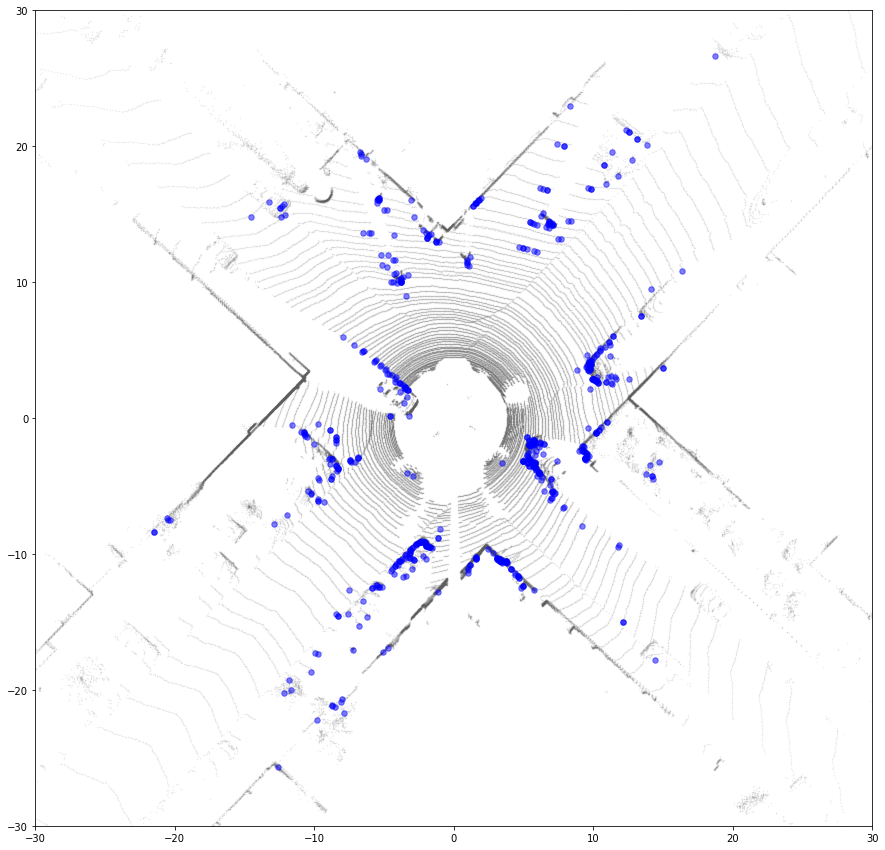
\includegraphics[width=\textwidth]{Figures/matching1.png}
         \captionsetup{font={small}} 
         \caption{}
         \label{fig:matching a}
     \end{subfigure}
     \begin{subfigure}[t]{0.25\textwidth}
         \centering
         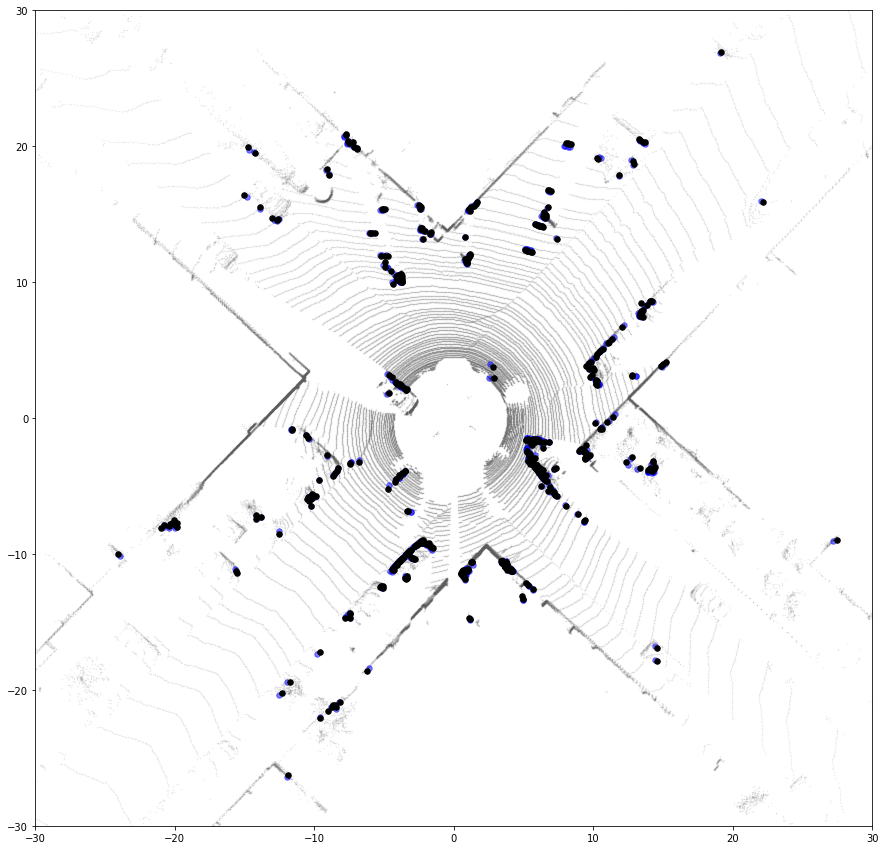
\includegraphics[width=\textwidth]{Figures/matching2.png}
         \captionsetup{font={small}} 
         \caption{}
         \label{fig:matching b}
     \end{subfigure}
     
        \caption{Illustration of MKPs detected by our methods. (a): The point cloud of $i+1$'s LiDAR scan, blue points are the keypoints detected by SIFT on the coordinate frame of  $i+1$'s scan. (b): Black points are the MKPs of the blue points from the $i's$ scan and projected to the $i+1's$ coordinate frame. The black points are expected to overlap to their paired blue points since they are match points projected to the same coordinate frame. Lines are aligned for each matched pair (blue point and paired black point). Here these lines are invisible because of overlapping. }
        \label{fig:matching3D}
\end{figure*}

%%%%%%%%%%%%%%%%%%%%%%%%%%%%%%%%%%%%%%%%%
% \newpage

\begin{figure*}[h]
  \centering
  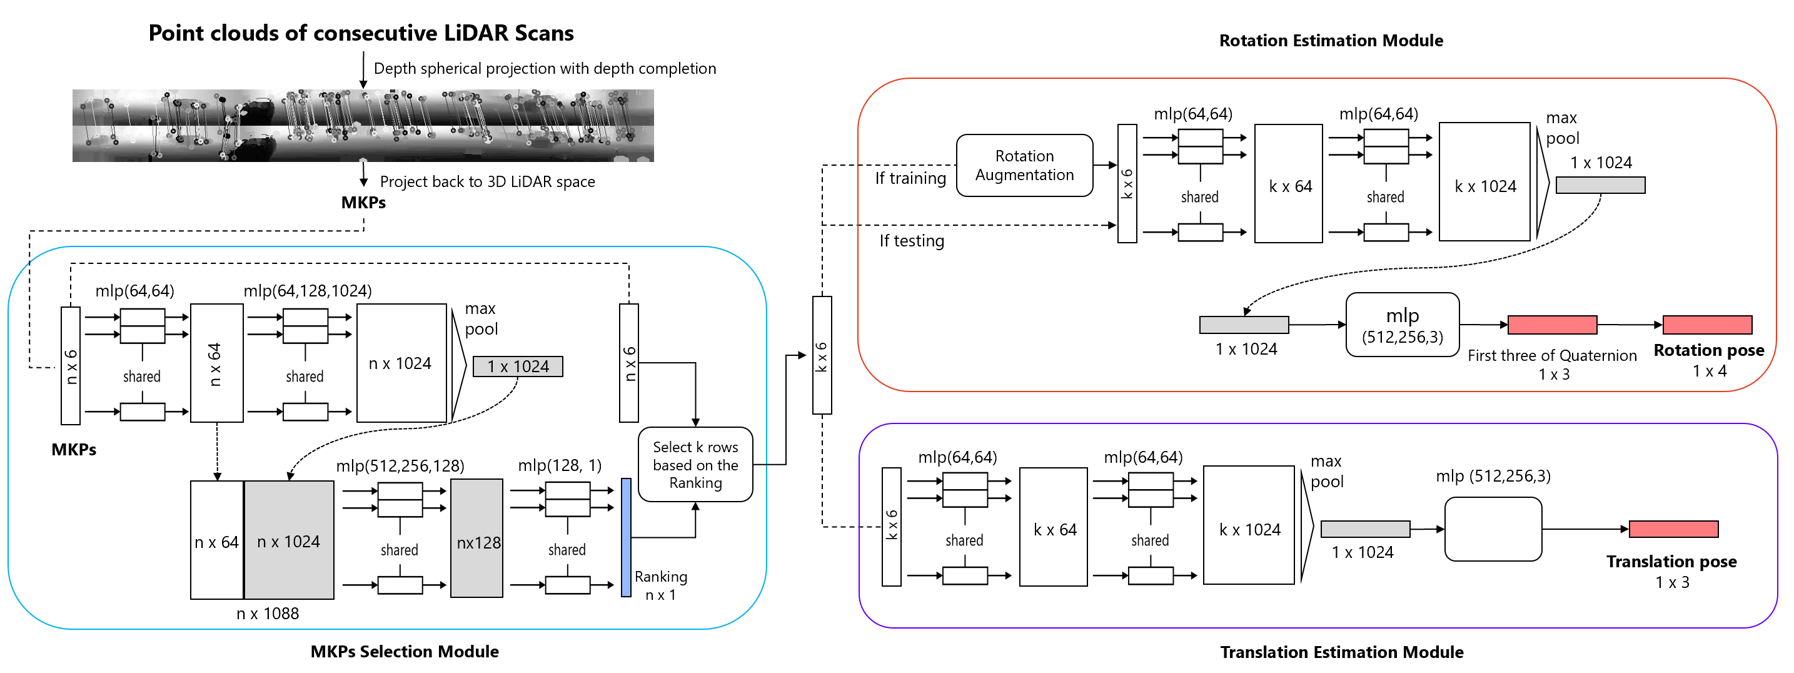
\includegraphics[height=0.32\textwidth]{Figures/network.png}
  \caption{\lodo{} Architecture:Depth spherical images of the LiDAR point clouds can be obtained by the projection procedure. The matching keypint pairs (MKPs) is extracted by the feature extraction algoritm:SIFT on the depth images than projected back to 3D LiDAR space. The MKPs Selection Module takes $n$ MKPs of consecutive scans as input. It can generate a Ranking Matrix $[n, 1]$ of the input $n$ MKPs, then we choose the best $k$ MKPs by their ranking as the input for rotation and translation estimation. The Rotation Estimation Module and Translation Estimation Module predict the rotation pose and translation pose respectively.Dotted line indicate two blocks are identical.}
  \label{fig:network}
\end{figure*}

\section{Related work}
\bfsection{LiDAR feature extraction in 2D space}

LiDAR feature extraction is one of the essential tasks of LiDAR-based applications. Since the raw data from the LiDAR sensors are not well structuralized and ordered, an intuitive way is to project the LiDAR points onto a 2D space. LoDNN \cite{caltagirone2017Lodnn} is a pioneering work that projects all LiDAR points onto the ground plane and samples them using an image-like array. In this work, however, the LiDAR points are not uniformly distributed on the ground plane but heavily gathered together near the LiDAR scanner, which results in massive dropped points in the near-range and redundant space in the far-range. Lyu \etal{} \cite{lyu2018real,lyu2018chipnet} and RangeNet++ \cite{milioto2019rangenet++} improve the projection scheme by replacing the target plane with a sphere surface, in which LiDAR points are nearly uniformly distributed. SqueezeSeg V1 \cite{wu2018squeezeseg}, V2 \cite{wu2019squeezesegv2}, and LO-Net \cite{LO-Net} also employ this projection scheme and result in a good performance in LiDAR point semantic segmentation. In our work, we follow the projection scheme of RangeNet++ to generate a 2D LiDAR feature map for each LiDAR frame.

\bfsection{Image feature extraction and keypoint detection}

Image feature extraction and keypoint detection have been studied for decades. Scale-invariant feature transform (SIFT) \cite{lowe1999sift} is one of the popular feature extraction algorithms in the image processing domain. By transforming an image into a large group of feature vectors that are invariant to image translation, scaling, and rotation, SIFT generates robust feature vectors on parts captured in different views. Other feature extraction methods include SURF \cite{bay2006surf} and ORB \cite{rublee2011orb}, however, they cannot generate robust feature vectors on LiDAR frames. In our work, we employ the SIFT as our LiDAR feature extractor.

\bfsection{Registration and feature-based vehicle odometry estimation}

Iterative Closet Point (ICP)\cite{ICP} method and its variants\cite{ICP_variants}\cite{ICP_variants1}\cite{ICP_variants2} have been used in the areas of LiDAR based pose estimation widely. In the ICP algorithm, a transformation between point clouds of adjacent scans is optimized iteratively by minimizing distance until a specific termination condition is met. Despite its popularity, ICP is sensitive to the initial poses and computationally expensive. Multiple variants of ICP algorithms such as point-to-line ICP\cite{ICP_l}, point-to-plane ICP\cite{ICP_p2plane}, and plane-to-pane ICP\cite{ICP_variants} were developed. GICP\cite{GICP} was proposed by combining point-to-point ICP and point-to-plane ICP into a single probabilistic framework. A probabilistic model is attached to the minimization step which can reduce the time complexity and increase the robustness to incorrect correspondences. Collar Line Segments (CLS)\cite{CLS} transforms the LiDAR scans into line could then generates line segments within each bin. This pre-processing method produces better results than GICP. However, due to the high computational cost in lien segments, CLS cannot achieve real-time odometry estimation. 

The state-of-art LiDAR Odometry estimation method: LiDAR Odometry And Mapping(LOAM)\cite{LOAM} was proposed by Zhang and Singh, which achieves both low-drift in motion estimation and low-computational complexity. The key idea is to divide the complex problem of Simultaneous Localization and Mapping into two parallel algorithms. One algorithm performs odometry at a high frequency but at low fidelity to estimate the velocity of the laser scanner. A second algorithm runs at an order of magnitude lower frequency for fine matching and registration of the point cloud.


\bfsection{Deep Learning-based vehicle odometry estimation}

In recent years, several works have been done exploring the use of neural networks in vehicle odometry estimation. DeepVO\cite{DeepVO}, DVSO\cite{DVSO}, Depth-VO-Feat\cite{Depth-VO-Feat}, and GANVO\cite{GANVO} have achieved promising results on Visual odometry(VO) estimation. In VO tasks, Camera data are used. However, applying Deep learning method to solve 3D LiDAR odometry problem still remains challenges. DeepICP\cite{Deep_icp} detects the keypoints by point weighting layer then generats a search region for each keypoint. A matched point can be generated by the corresponding point generation layer. The final registration computes by SVD given the matched keypoints pairs. DeepPCO\cite{DeepPCO} generates panormaic-view of depth image projection to feed to it neural networks. L3-Net \cite{lu2019l3} proposes a learning-based LiDAR localization system by comparing the network-based feature vector between the current LiDAR frame and pre-build point cloud map followed by a recurrent neural network based smoothness module. LO-Net\cite{LO-Net} is another learning-based odometry estimator. Different from L3-Net that only extracts point-wise features, LO-Net  projects the points on a sphere surface and build an image-like feature map for each LiDAR frame. For better training the odometry estimator, LO-Net introduces an attention branch to predict if the geometric consistency of an area in the feature map can be modeled or not. In contrast to those learning-based algorithms using networks to extract features and estimate the odometry. 

\section{Method}
\subsection{Problem Setup}

We are given a collection of training samples $\{(\mathcal{X}_t, \mathcal{X}_{t+1}, \mathbf{y}_{t})\}_{t\in\mathcal{T}}$ where $\mathcal{X}_t\subseteq\mathbb{R}^3$ denotes the set of keypoints from the $t$-th \lidar{} scans, $\mathbf{y}_{t}\in\mathcal{Y}\subseteq\mathbb{R}^6$ denotes the ground-truth odometry between the $t$-th and $(t+1)$-th \lidar{} scans, and $\mathcal{T}$ denotes the scan index set. Our goal is to learn an odometry prediction function $f:\mathcal{X}\times\mathcal{X}\rightarrow\mathcal{Y}\in\mathcal{F}$ by minimizing certain loss function $\ell:\mathcal{Y}\times\mathcal{Y}\rightarrow\mathbb{R}$, \ie
\begin{align}\label{eqn:general}
% \setlength{\abovedisplayskip}{5pt}
% \setlength{\belowdisplayskip}{5pt}
% \setlength{\abovedisplayshortskip}{5pt}
% \setlength{\belowdisplayshortskip}{5pt}
% \small
    \min_{f\in\mathcal{F}}\sum_{t\in\mathcal{T}}\ell(f(\mathcal{X}_t, \mathcal{X}_{t+1}), \mathbf{y}_{t}).
\end{align}
Note that Eq. \ref{eqn:general} holds in general for all the \lidar{} odometry estimation algorithms. To simplify our explanation later, here we assume that the feasible space $\mathcal{F}$ is proper, closed, and convex (PCC) that covers all the constraints on $f$ such as regularization. At test time, given two sets of keypoints $\mathcal{X}_{t'}, \mathcal{X}_{t'+1}$, we can predict their odometry as $f(\mathcal{X}_{t'}, \mathcal{X}_{t'+1})$.


\subsection{Formulation}

As we know, odometry has 6 degrees of freedom (DOF). This leads to the fact that odometry can be estimated given at least 3 matched keypoint pairs (MKPs). Therefore, instead of learning the general function $f$ in Eq. \ref{eqn:general} directly, in the literature it will be more plausible to decompose it as two functions, \ie $f=h\circ g$ where $\circ$ denotes the function composition. The keypoint matching function, $g:\mathcal{X}_t\times\mathcal{X}_{t-1}\rightarrow\mathcal{P}_{t}\times\mathcal{P}_{t-1}\subseteq\mathbb{R}^3\times\mathbb{R}^3$, generates MKPs from the input keypoint sets, and the odometry regression function, $h:\mathcal{P}_t\times\mathcal{P}_{t-1}\rightarrow\mathcal{Y}$, predicts the odometry based on the MKPs. Odometry estimation algorithms are all about how to design or learn such functions $g, h$ to determine function $f$.

\bfsection{ICP-based learning approaches}
Iterative Closest Point (ICP) \cite{besl1992method} matches two sets of points iteratively as well as estimating the pose transformation by minimizing distances between the corresponding matched points until it converges. Although ICP is well-known for point registration, the high computation and sensitivity to initial poses significantly limit its applications. The key idea behind ICP-based learning approaches for \lidar{} odometry estimation is to use ICP to locate MKPs (given the current odometry regression function $h$) that are used to update $h$ further. In general, such approaches can be formulated as follows:
\begin{align}\label{eqn:ICP}
\small
    \min_{h\in\mathcal{H}} \sum_{t\in\mathcal{T}}\ell(h(\mathcal{P}_{t}, \mathcal{P}_{t+1}), \mathbf{y}_{t}), 
    s.t. \; \mathcal{P}_{t}, \mathcal{P}_{t+1} = \Tilde{g}(\mathcal{X}_{t}, \mathcal{X}_{t+1}, h(\mathcal{P}_{t}, \mathcal{P}_{t+1})) %\; d(q(\mathcal{P}_{t,i}, h(\mathcal{P}_{t}, \mathcal{P}_{t+1})), \mathcal{P}_{t+1,i}) \leq \epsilon, \forall i\in[|\mathcal{P}_t|], \nonumber
\end{align}
where $\tilde{g}:\mathcal{X}\times\mathcal{X}\times\mathcal{Y}\rightarrow\mathcal{P}\times\mathcal{P}$ denotes a variant of the keypoint matching function, and the feasible space $\mathcal{H}$ is PCC. 

The constraint here models the MKPs as the stationary solution given current $h$, which can be viewed as a generalization of ICP. Then such solutions are used to update $h$ in the objective by minimizing the loss. At training time this procedure is repeated until it converges. At test time, given $\tilde{g}$ and learned $h$ we use the constraint to locate the MKPs and then output the odometry estimation as $h(\mathcal{P}_{t'}, \mathcal{P}_{t'+1})$. %Alg. \ref{alg:ICP} summarizes the training and testing procedures above.



\begin{align}\label{eqn:ICP_PQ}
\small
    \mathbf{Q}_i=
    \begin{bmatrix}
        x_{i,1}^2+x_{i,2}^2 & -x_{i,2}x_{i,3} & -x_{i,1}x_{i,3} & x_{i,2} & -x_{i,1} & 0 \\
        -x_{i,2}x_{i,3} & x_{i,1}^2+x_{i,3}^2 & -x_{i,1}x_{i,2} & -x_{i,3} & 0 & x_{i,1} \\
        -x_{i,1}x_{i,3} & -x_{i,1}x_{i,2} & x_{i,2}^2+x_{i,3}^2 & 0 & x_{i,3} & -x_{i,2} \\ 
        x_{i,2} & -x_{i,3} & 0 & 1 & 0 & 0 \\
        -x_{i,1} & 0 & x_{i,3} & 0 & 1 & 0 \\
        0 & x_{i,1} & -x_{i,2} & 0 & 0 & 1
    \end{bmatrix}
\end{align}

\begin{align}
\small
    \mathbf{q}_i = 
    \begin{bmatrix}
        y_{i,1}x_{i,2} - y_{i,2}x_{i,1} \\
        -y_{i,1}x_{i,3} + y_{i,3}x_{i,1} \\
        y_{i,2}x_{i,3} - y_{i,3}x_{i,2} \\
        x_{i,1} - y_{i,1} \\
        x_{i,2} - y_{i,2} \\
        x_{i,3} - y_{i,3}
    \end{bmatrix}
\end{align}

\begin{align}
\small
    \begin{bmatrix}
        \alpha\\
        \beta\\
        \gamma\\
        b_1\\
        b_2\\
        b_3
    \end{bmatrix}=-\left[\sum_i\mathbf{Q}_i\right]^{-1}\sum_i\mathbf{q}_i
\end{align}


\bfsection{Our \lodo{}}
As we see in Eq. \ref{eqn:ICP}, the odometry regression function $h$ and the keypoint matching function $g$ in ICP-based learning approaches are essentially {\em coupled}. This potentially can lead to two serious problems, at least, in training, \ie high computation and non-convergence of the training loss.

To address such problems, our methodology in \lodo{} is to decouple functions $g, h$ to avoid the loop as well as significantly improving the convergence. To this end, we propose the following optimization problem:
\begin{align}\label{eqn:lodonet}
\small
    \min_{z\in\mathcal{Z},  \Tilde{h}\in\tilde{\mathcal{H}}}  \sum_{t\in\mathcal{T}}\ell & (\tilde{h}(\mathcal{P}_{t},  \mathcal{P}_{t+1}, z(\mathcal{P}_{t}, \mathcal{P}_{t+1})), \mathbf{y}_{t}), \; \notag \\
    s.t. \;& \mathcal{P}_{t}, \mathcal{P}_{t+1} = g(\mathcal{X}_{t}, \mathcal{X}_{t+1}), 
\end{align}
where $z:\mathcal{P}\times\mathcal{P}\rightarrow\Pi$ denotes an {\em attentional} function that returns probability vectors over the MKPs in the simplex space $\Pi$, $\tilde{h}:\mathcal{P}\times\mathcal{P}\times\Pi\rightarrow\mathcal{Y}$ denotes a variant of the odometry regression function, and both spaces $\mathcal{Z}, \tilde{H}$ are PCC.

Different from ICP-based learning approaches, here we use a predefined keypoint matching function $g$ to extract MKPs from \lidar{} data (\ie constraint), and feed these MKPs as input to the learning algorithm directly to minimize the objective. In this way, there is no loop between $g$ and $\tilde{h}$ (\ie decoupling). The quality of the MKPs, however, cannot be guaranteed to be good for odometry estimation. Therefore, we deliberately introduce the attentional mechanism to assign weights for estimation. In fact, Eq. \ref{eqn:lodonet} is an unconstrained minimization problem with convergence guarantee using alternating optimization (\ie learning $z$ while fixing $\tilde{h}$, and then learning $\tilde{h}$ while fixing $z$), in general, as $(\mathcal{P}_t, \mathcal{P}_{t+1}), \forall t\in\mathcal{T}$ now are the inputs. At test time we predict the odometry as $\tilde{h}(\mathcal{P}_{t}, \mathcal{P}_{t+1}, z(\mathcal{P}_{t}, \mathcal{P}_{t+1}))$.

\subsection{Data prepossessing}
\label{section:Data prepossessing}

% \begin{figure}[h]
%   \centering
%   \includegraphics[width=\linewidth]{Figures/spherical image.png}
%   \caption{The spherical image of one LiDAR scan}
%   \label{fig:spherical}
% \end{figure}

\begin{figure*}[h]
     \centering
     
     \begin{subfigure}[b]{0.9\textwidth}
         \centering
         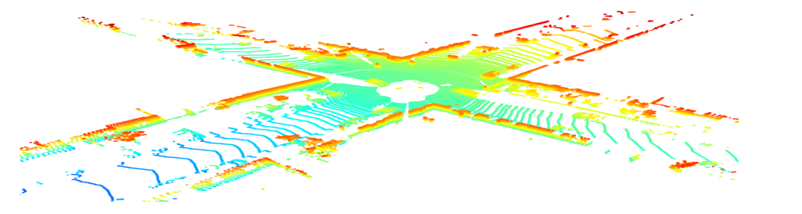
\includegraphics[width=0.4\textwidth]{Figures/lidar point.png}
         \captionsetup{font={scriptsize}} 
         \caption{Point Cloud of one LiDAR scan}
         \label{fig:spherical a}
     \end{subfigure}
    
     \begin{subfigure}[b]{0.8\textwidth}
         \centering
         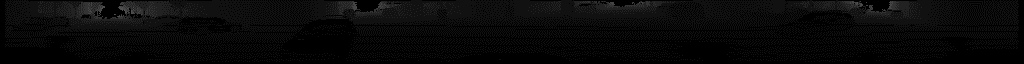
\includegraphics[width=\textwidth]{Figures/spherical image b.png}
         \captionsetup{font={scriptsize}} 
         \caption{Original spherical image of one scan of LiDAR Point}
         \label{fig:spherical b}
     \end{subfigure}
     
     \begin{subfigure}[b]{0.8\textwidth}
         \centering
         
\includegraphics[width=\textwidth]{Figures/spherical image c.png}
         \captionsetup{font={scriptsize}} 
         \caption{Depth spherical image of the original spherical image}
         \label{fig:spherical c}
     \end{subfigure}
     

     \begin{subfigure}[b]{0.8\textwidth}
         \centering
         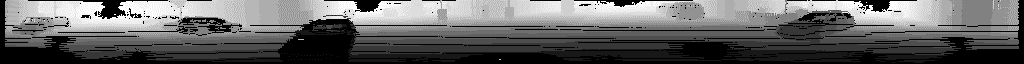
\includegraphics[width=\textwidth]{Figures/spherical image d.png}
         \captionsetup{font={scriptsize}} 
         \caption{Histogram equalization of the original spherical image}
         \label{fig:spherical d}
     \end{subfigure}
     
     \begin{subfigure}[b]{0.8\textwidth}
         \centering
         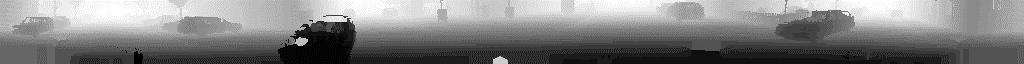
\includegraphics[width=\textwidth]{Figures/spherical image e.png}
         \captionsetup{font={scriptsize}} 
         \caption{Histogram equalization of the depth completion spherical image}
         \label{fig:spherical e}
     \end{subfigure}
     
        \caption{The spherical image of one LiDAR scan}
        \label{fig:spherical}
\end{figure*}


\bfsection{Depth spherical image generation from LiDAR point clouds}

The 3D LiDAR point clouds are usually stored by a set of Cartesians
coordinates $(X, Y, Z)$. Due to the relative low resolution of LiDAR scanners, the 3D LiDAR point clouds are quite sparse. A scan of the LiDAR point cloud is shown in Fig \ref{fig:spherical a}. However, matching keypoints pairs from two consecutive scans of LiDAR point clouds would be inaccurate and time/memory consuming. Therefore, we project the sparse LiDAR point clouds into spherical projection images, which is a relative dense representation. The projection function is: 

\begin{align}
\small
    \alpha = \arcsin(\frac{z}{\sqrt{x^2 + y^2 +z^2}}), \; 
    \Bar{\alpha} = | \frac{\alpha}{	\Delta\alpha} |
\end{align}

\begin{align}
\small
    \beta = \arcsin(\frac{y}{\sqrt{x^2 + y^2}}), \;
    \Bar{\beta} = | \frac{\beta}{	\Delta\beta} |
\end{align}
Where $\alpha$ and $\beta$ are the indexes of points' position in the matrix. $\Delta\alpha$ and $\Delta\beta$ are the angular resolutions in the horizontal and vertical directions, respectively. The element at $(\alpha, \beta)$ of the spherical image is set to be the range value $r = \sqrt{x^2 + y^2 +z^2} $ of the LiDAR point $(x, y, z)$ \cite{LO-Net}. A matrix of size $H \times W \times C$ can be obtained by applying this projection. $H$ is the number of vertical channels from LiDAR scanners, $W$ is the width of the spherical image, and $C$ is the channel of input point cloud matrix. Fig \ref{fig:spherical b} shows the spherical image of one LiDAR scan (Fig \ref{fig:spherical a}). 


\bfsection{Depth completion and histogram equalization}

In depth completion we aim to fill the void pixels in our projected spherical image, so that every pixel can be utilized in the following algorithms. Traditional image inpainting algorithms try to interpolate the target pixels using surrounding pixel color values, which is computational expensive for real-time processing. In this paper, based on the assumption that depth value does not change much in local regions, we speed up the depth completion by filling the void pixels with the depth value of its nearest valid pixels. The algorithm is described in algorithm \ref{alg:Depth Completion}. 
\begin{algorithm}[t]\footnotesize
	\SetAlgoLined
	\begin{flushleft}

     \textbf{INPUT:} valid pixel set $\mathcal{P}_1 = \{\mathbf{p}_1\}$, void pixel set $\mathcal{P}_0 = \{\mathbf{p}_0\}$\\
	 \textbf{OUTPUT:} filled pixel set $\mathcal{P}_0 = \{\mathbf{p}_0\}$\\
	\end{flushleft}
    \begin{algorithmic}[1]
    \State \textbf{For Each} $\mathbf{p}_0$ in $ \mathcal{P}_0 $:
    \State \quad  $\mathbf{p}' \in \argmin_{\mathbf{p}_1\in \mathcal{P}_1}\left\{||\mathbf{p}_0 - \mathbf{p}_1||\right\}$
,   \State \quad  $\mathbf{p}_0 \leftarrow \mathbf{p}^*$
    \State \textbf{End}
    \State Return $\mathcal{P}_0$
    
    \end{algorithmic}
	\caption{\footnotesize Depth Completion}\label{alg:Depth Completion}
\end{algorithm}



As shown in the Figure ~\ref{fig:spherical b}, the value in each pixel represents the distance of the original LiDAR detected point to the LiDAR that causes the most pixels in the spherical image to have a relatively small value. To improve the spherical image’s visual quality, we apply the histogram equalization technique in order to enhance the contrast as shown in Figure ~\ref{fig:spherical c}. Histogram equalization is the most popular contrast enhancement technique due to simplicity and effectiveness \cite{2008digital}. This widely used technique achieved by flattening the dynamic range of an image’s histogram of grey value based on the probability density function \cite{contrastenhancement}. After we generate the depth completion spherical image in Figure ~\ref{fig:spherical d} , we apply the Histogram equalization. Therefore, the brightness of the depth completion spherical image is improved significantly as shown in the Figure ~\ref{fig:spherical e}.

\bfsection{Keypoints detection and matching}

After the depth completion and histogram equalization step, we want to detect a group of MKPs from consecutive frames of spherical images $f_i$ and $f_{i+1}$. For example, one keypoint is shown in $f_i$ at the location $(x_1, y_1)$  and its matching point is located at $({x_1}^\prime, {y_1}^\prime)$ in $f_{i+1}$. Since this MKP represent the same object in consecutive images of frames, the potential odometry information between these consecutive frames is related to their location in spherical images. Thus, we apply the SIFT algorithm to detect keypoints in consecutive frames of spherical images. This local feature extraction method can extract comprehensive keypoints which are invariant to the object translation and rotation. Each detected keypoint will be represented as a 128$-$element vector, called by descriptors \cite{whensift}. The features of descriptors will be used for keypoint matching.

Given a keypoint from depth completion image  $f_i$, we want to find the best match point in $f_{i+1}$ to form the MKP. The similarity will be measured based on the feature matching algorithm of calculating the Euclidean distance between keypoints in the spherical image \cite{siftvo}. In Figure ~\ref{fig:MKPs} (a), two consecutive scans are concatenated vertically. The Figure ~\ref{fig:MKPs} (b) shows the top 400 MKPs detected from these consecutive scans. However, some MKPs are mismatched or not suitable for odometry estimation. For example, we do not want to use any point from dynamic objects. Figure ~\ref{fig:MKPs} (c) illustrates the 100 MKPs selected by MKP Selection module among the 1000 MKPs detected in this section. We will discuss this issue in section \ref{section:train lodo}.

\begin{figure*}[h]
     \centering
     \begin{subfigure}[b]{0.8\textwidth}
         \centering
         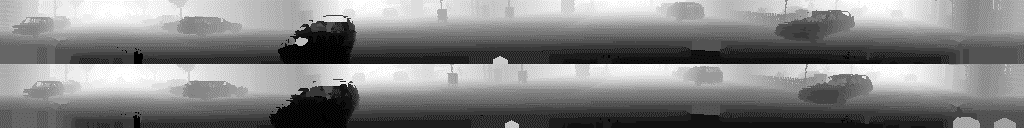
\includegraphics[width=\textwidth]{Figures/MKP a.png}
         \captionsetup{font={small}} 
         \caption{2 consecutive frames of LiDAR scans}
        %  \label{fig:spherical b}
     \end{subfigure}

     \begin{subfigure}[b]{0.8\textwidth}
         \centering
         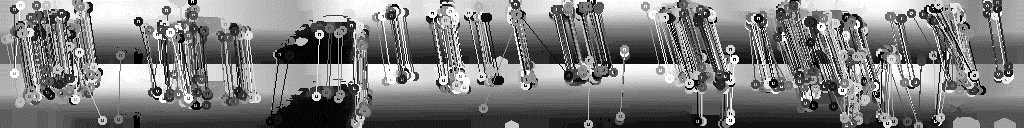
\includegraphics[width=\textwidth]{Figures/MKP b.png}
         \captionsetup{font={small}} 
         \caption{Top 400 MKPs detected by SIFT}
     \end{subfigure}
     
     \begin{subfigure}[b]{0.8\textwidth}
         \centering
         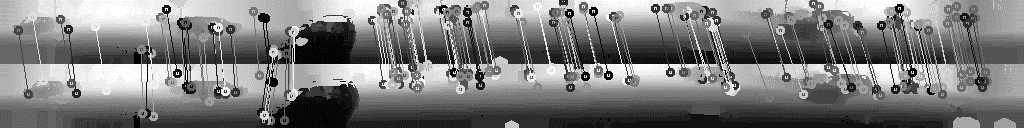
\includegraphics[width=\textwidth]{Figures/MKP c.png}
         \captionsetup{font={small}} 
         \caption{100 MPKs selected by MKPs Selection Module}
     \end{subfigure}
     
        \caption{MKPs extracted from consecutive LiDAR scans}
        \label{fig:MKPs}
\end{figure*}

% \begin{figure}[h]
%   \centering
%   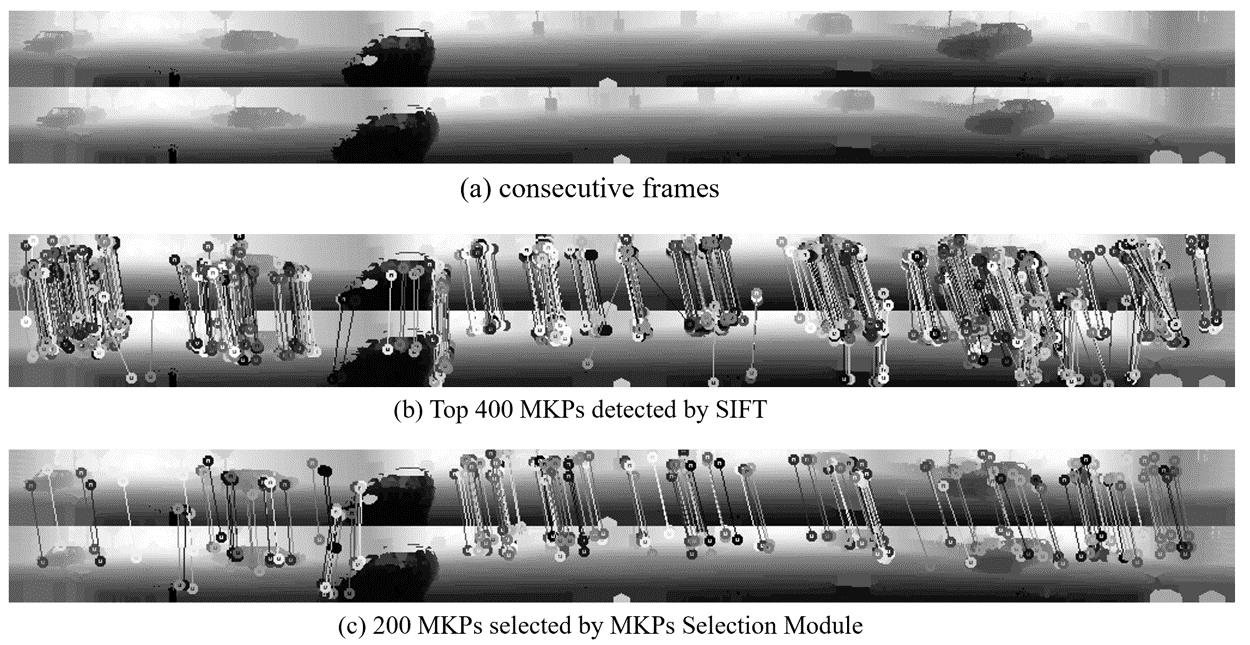
\includegraphics[width=\linewidth]{Figures/MKP.png}
%   \caption{MKPs of consecutive frames}
%   \label{fig:MKPs}
% \end{figure}

\bfsection{Projecting back to 3D point cloud}

It is simple to project MKPs in the spherical image back to 3D point clouds. Noticed that the MKPs were detected from depth completion spherical image, some MKPs may not have corresponding points in the original 3D space. In other words, some “fake” MKPs are generated by depth completion, not from original LiDAR points. These “fake” MKPs are removed and only real MKPs return the points coordinate in 3D space. The MKPs which related to the odometry rotation and translation are extracted from entire LiDAR points of consecutive frames. Then we aligned the points in frame $f_i$ with their matching points in frame $f_{i+1}$ to construct a matrix with the size of $[m , 6]$ where $m$ is the number of MKPs we find, and 6 is the x, y, z coordinate of matching points in consecutive frames. 

\subsection{LiDAR odometry regression}
\label{section:train lodo}
\bfsection{MKPs Selection module}

In section \ref{section:Data prepossessing}, we extract MKPs of consecutive frames which relative to the odometry rotation and translation information. However, some of MKPs are inappropriate for estimating odometry. We want to exclude those MKPs from dynamic objects such as moving cars. Even though matching are good, these MKPs may inhibit the odometry estimation due to the inconsistence odometry information of dynamic objects with LiDAR device. Hence a selection module is needed to determine whether a matching point should be used for odometry estimation. 

we deploy a MKPs Selection module to solve this segmentation problem in order to improve the effectiveness and robustness of the network. Here we use the PointNet segmentation structure to achieve the goal. The PointNet consists of symmetry function for unordered input, a local and global information aggregation, and a joint alignment network. In our MKPs Selection module, we modify several parts to fit our scenario. T-Net structure has been removed since we don't want to preserve the rotation invariant. The input are MKPs of consecutive frames, not original unordered points. For the output $M_S(P_i) \in [0,1]$, ground truth odometry which containing rotation $R$ and translation $T$ information are used to calculate the distance of the point in frame i with its matching point’s projection in frame i by the following equation: 
\begin{align}
\small
    d =\| \begin{bmatrix}
            R & T \\
            0 & 1 
            \end{bmatrix}  \mathcal{X}_i - \mathcal{X}_{i+1} \|_2 
\end{align}
The output is set as 1 if the distance is small while large distance indicates the output is 0. MKPs with label 1 will be use in the odometry estimation.

\bfsection{Rotation Estimation module}

\begin{algorithm}[t]\footnotesize

	\SetAlgoLined
	\begin{flushleft}
    \textbf{INPUT:} Point cloud pair $\mathcal{P}_1,\mathcal{P}_2$, odometry Matrix Ground Truth $Tr$, augmentation rotation upper-bound $beta_{max}$ \\
	\textbf{OUTPUT:} Augmented point cloud pair $\mathcal{P}'_1,\mathcal{P}'_2$, augmented odometry Matrix Ground Truth $Tr'$ \\ 
	\end{flushleft}
    \begin{algorithmic}
    \State$\beta \leftarrow Random(-\beta_{max},\beta_{max})$
    \State$Tr1 \leftarrow Yaw(\beta)$
    \State$Tr' \leftarrow [Tr]^{-1}\mathcal{P}_2$
    \State$\mathcal{P}'_1 \leftarrow \mathcal{P}_1$
    \State$\mathcal{P}'_2 \leftarrow Tr1 \mathcal{P}_1$
    \State Return $\mathcal{P}'_1,\mathcal{P}'_2,Tr'$
    \end{algorithmic}
	\caption{\footnotesize Data Augmentation on Odometry Rotation}\label{alg:augmentation}
\end{algorithm}

After selecting a fixed number of MKPs, we aim to infer the 3-DoF relative odometry rotation information by constructing a regression model. By observing popular autonomous driving datasets with LiDAR odometry task, recording cars usually go straight line while turning frames are not enough. Hence, we apply a data augmentation procedure for rotation estimation. Because each matching pair associate with the 3-DoF odometry rotation information R, the Equation \ref{eqn:ICP_PQ} represents the relation between matching pairs with a rotation matrix. We can generate the augmented MKPs with corresponding rotation matrix by given the existing MKPs with their rotation matrix based on the algorithm \ref{alg:augmentation}.

The structure of rotation estimation module is based on the PointNet classification model while we change it to the regression model. We remove the T-net structure and add our rotation augmentation structure. The input of the Rotation Estimation module is selected MKPs from the MKPs Selection module concatenate with rotation augmentation of selected MKPs. The output is the Unit Quaternion format of the odometry rotation information. The Unit Quaternion of two consecutive frames can be represented by a vector $[a, bi, cj, dk]$, where a, b, c, and d are real numbers, and i, j, and k are the fundamental Quaternion units \cite{Quaternion}. Based on the norm of the Unit Quaternion vector is equal to 1, here we only predict the first three dimension of Unit Quaternion and the last dimension can be calculated afterwards. 
The rotation loss function of consecutive frames is defined as: 
\begin{align}
\small
    \mathcal{L}_R =\|  Q - \hat{Q} \|_l 
\end{align}
Where $Q$ is the ground truth first three dimension of Unit Quaternion, $\hat{Q}$ is the predicted first three dimension of Unit Quaternion by the network, and $l$ refers to the Euclidean distance norm. Here we choose the $l_2$ norm in this module. 

\bfsection{Translation Estimation module}

The network structure of Translation estimation module is quite similar to the Rotation Estimation module. In contrast, we directly apply the selected MKPs as input to feed the Translation Estimation module since the translation augmentation is not required. The output is the 3-DoF odometry translation information and the loss function is defined as: 
\begin{align}
\small
    \mathcal{L}_T =\|  T - \hat{T} \|_l 
\end{align}
Where $T$ is the ground truth translation matrix, $\hat{T}$ is the predicted translation array by the network, and $l$ refers to the Euclidean distance norm. Here we choose the $l_2$ norm in this module. 

\section{Experiments}
\subsection{Implementation detail}
\label{section:Implementation detail}
In our experiment, we only use the point cloud data which is collected by the Velodyne HDL-64 3D LiDAR sensor to estimate the odometry. When converting LiDAR point cloud to spherical image, we set the height of the image as 64 and the width as 1024. For each two consecutive scans $f_i$ and $f_{i+1}$, we detect MKPs on spherical images then convert back to 3D space. In a sequence of point clouds with $n+1$ scans, we can collect 1000 MKPs for $n$ consecutive frames to form an input matrix $[n, 1000, 6]$. \lodo{} predicts the odometry between n consecutive frames and give an output as $[n, 7]$, then we can calculate the odometry matrix $[n, 12]$ indicating each scan’s odometry by the relation of rotation and translation matrix. The whole framework is implemented with the Tensorflow, we choose the Adam optimizer\cite{adam} for optimization. The batch size and learning rate are set to be 128 and 0.0001. MKPs Selection module select 100 MKPs among 1000 MKPs for each consecutive scans. One GeForce RTX 2080 Ti GPU is used for training. 

\subsection{Dataset}

\quad \textbf{KITTI}. The KITTI odometry dataset\cite{kitti} is a popular and widely used dataset in the autonomous driving tasks. It provides 22 independent sequences with stereo gray-scale camera images, color camera images, and point clouds captured by a Velodyne HDL-32 LiDAR sensor among urban, highway and countryside scenes. For our work, we only use Velodyne LiDAR data to estimate odometry. For sequence 0 to sequence 10, KITTI dataset provides the ground truth odometry while the ground truth odometry for sequence 11 to sequence 21 is not available. Hence, we use sequence 0, 1, 2, 3, 4, 5, 6, 9, and 10 to train our model while leaving sequence 7 and sequence 8 for testing. 


As we state in section \ref{section:train lodo} that odometry has 6 degrees of freedom which can be represented by rotation and translation components. In the ground-truth odometry pose files provided by KITTI dataset, a 12 by 1 vector is assigned for the odometry pose of $i_{th}$ frame to the 0 frame while 9 of them indicating the rotation and 3 of them present the translation. This 9-dimension rotation vector usually reshapes to a 3 by 3 rotation matrix. In our experiments, we convert this 3 by 3 rotation matrix to a 1 by 4 Unit Quaternion representation due to less dimension for network training. Noted here we only predict first three dimension of Unit Quaternion and the last dimension can be calculated due to the norm of the Unit Quaternion is euqal to 1. Thus, given the input of the MKPs of two consecutive frames, the output of our network is a 1 by 7 vector which is concatenated by a 1 by 4 rotation vector with a 1 by 3 translation vector.

\subsection{Evaluation}
We compared our method with the ground truth trajectory and several LiDAR odometry estimation methods: ICP-point2point(ICP-po2po), ICP-point2plane (ICP-po2pl), GICP\cite{GICP}, CLS\cite{CLS}, LOAM\cite{LOAM}, Velas et al.\cite{Velas}, LO-Net\cite{LO-Net}.

\begin{table*}
\centering
  \caption{Odometry results on KITTI dataset}
  \resizebox{0.9\textwidth}{!}{
\begin{tabular}{|c|cccccccccccccccccc|cc|}
\hline
                      & \multicolumn{2}{c}{ICP-po2po} & \multicolumn{2}{c}{ICP-po2pl} & \multicolumn{2}{c}{GICP\cite{GICP}} & \multicolumn{2}{c}{CLS\cite{CLS}} & \multicolumn{2}{c}{LOAM\cite{LOAM}}      & \multicolumn{2}{c}{Velas et al\cite{Velas}} & \multicolumn{2}{c}{DeepPCO\cite{DeepPCO}} & \multicolumn{2}{c}{LO-Net\cite{LO-Net}} & \multicolumn{2}{c|}{ours}                                 \\ \cline{2-19} 
\multirow{-2}{*}{seq} & t\_rel        & r\_rel        & t\_rel        & r\_rel        & t\_rel  & r\_rel         & t\_rel     & r\_rel     & t\_rel        & r\_rel        & t\_rel         & r\_rel         & t\_rel       & r\_rel       & t\_rel          & r\_rel   & t\_rel                      & r\_rel                      \\ \hline
00                    & 6.88          & 2.99          & 3.80          & 1.73          & {\color[HTML]{3531FF} 1.29}    & {\color[HTML]{3531FF} 0.64}           & 2.11       & 0.95       & \textbf{0.78} & \textbf{0.53} & 3.02           & /              & /            & /            & 1.47            & 0.72     & 1.43 & 0.69 \\
01                    & 11.21         & 2.58          & 13.53         & 2.58          & 4.39    & 0.91           & 4.22       & 1.05       & 1.43          & 0.55          & 4.44           & /              & /            & /            & {\color[HTML]{3531FF} 1.36}            & {\color[HTML]{3531FF} 0.47}    & \textbf{0.96}               & \textbf{0.28}               \\
02                    & 8.21          & 3.39          & 9.00          & 2.74          & 2.53    & 0.77           & 2.29       & 0.86       & \textbf{0.92} & \textbf{0.55} & 3.42           & /              & /            & /            & 1.52            & 0.71     & {\color[HTML]{3531FF} 1.46} & {\color[HTML]{3531FF} 0.57} \\
03                    & 11.07         & 5.05          & 2.72          & 1.63          & 1.68    & 1.08           & 1.63       & 1.09       & \textbf{0.86} & \textbf{0.65} & 4.94           & /              & /            & /            & {\color[HTML]{3531FF} 1.03}            & {\color[HTML]{3531FF} 0.66}     & 2.12                        & 0.98                        \\
04                    & 6.64          & 4.02          & 2.96          & 2.58          & 3.76    & 1.07           & 1.59       & 0.71       & 0.71          & {\color[HTML]{3531FF} 0.50}          & 1.77           & /              & 2.84         & 3.07         & \textbf{0.51}   & 0.65     &  {\color[HTML]{3531FF} 0.65}                        & \textbf{0.45}               \\
05                    & 3.97          & 1.93          & 2.29          & 1.08          & {\color[HTML]{3531FF} 1.02}    & {\color[HTML]{3531FF} 0.54}            & 1.98       & 0.92       & \textbf{0.57} & \textbf{0.38} & 2.35           & /              & /            & /            &   1.04           & 0.69     & 1.07                        & 0.59 \\
06                    & 1.95          & 1.59          & 1.77          & 1.00          & 0.92    & 0.46           & 0.92       & 0.46       & {\color[HTML]{3531FF} 0.65}          & {\color[HTML]{3531FF} 0.39}          & 1.88           & /              & /            & /            & 0.71            & 0.50     & \textbf{0.62}               & \textbf{0.34}               \\
07                    & 5.17          & 3.35          & 1.55          & 1.42          &  {\color[HTML]{3531FF} 0.64}    & \textbf{0.45}  & 1.04       & 0.73       & \textbf{0.63} & {\color[HTML]{3531FF} 0.50}          & 1.77           & /              & /            & /            & 1.70            & 0.89     & 1.86                        & 1.64                        \\
08                    & 10.04         & 4.93          & 4.42          & 2.14          &  {\color[HTML]{3531FF} 1.58}    & {\color[HTML]{3531FF} 0.75}           & 2.14       & 1.05       & \textbf{1.12} & \textbf{0.44} & 2.89           & /              & /            & /            & 2.12            & 0.77     & 2.04 & 0.97                        \\
09                    & 6.93          & 2.89          & 3.95          & 1.71          & 1.97    & 0.77           & 1.95       & 0.92       & {\color[HTML]{3531FF} 0.77}          & {\color[HTML]{3531FF} 0.48}          & 4.94           & /              & /            & /            & 1.37            & 0.58     & \textbf{0.63}               & \textbf{0.35}               \\
10                    & 8.91          & 4.74          & 6.13          & 2.60          & 1.31    & 0.62           & 3.46       & 1.28       & \textbf{0.79} & {\color[HTML]{3531FF} 0.57}          & 3.27           & /              & 2.41         & 6.70         & 1.80            & 0.93     & {\color[HTML]{3166FF} 1.18} & \textbf{0.45}               \\ \hline
aveage                & 7.36          & 3.41          & 4.74          & 1.93          & 1.92    & 0.73           & 2.12       & 0.91       & \textbf{0.84} & \textbf{0.46} & 3.15           & /              & /            & /            & 1.33            & 0.69     & {\color[HTML]{3166FF} 1.27} & {\color[HTML]{3166FF} 0.66} \\ \hline
\end{tabular}}
\label{tab:results}
\end{table*}


Table 1 shows the evaluation results of the mentioned methods on the KITTI dataset. We use $t_{rel}$: the Average Translational RMSE($\%$) and $r_{rel}$: Average Rotational RMSE($^\circ$/100m) to evaluate the results of different methods. There are few deep learning-based approaches for LiDAR odometry estimation that have comparable results. DeepPCO\cite{DeepPCO} only reports the results on its validation sequences. However they did not specify the unit of $t_{rel}$ and $r_{rel}$. Based on the trajectories they provide, we determine that their $t_{rel}$ is 2.63 and $r_{rel}$ is 3.05 for sequence 04, and  $t_{rel}$ is 2.47 and $r_{rel}$ is 6.59 for sequence 10 with the same unit as in Table ~\ref{tab:results}. CAE-LO\cite{CAE-LO} 
did not provide the results on KITTI Seq 00-10. LO-Net\cite{LO-Net} is one of the best deep learning methods for LiDAR Only Odometry estimation. From Table ~\ref{tab:results}, The Seq 07 and 08 ate not used to train \lodo{}. Bold number indicates the best performance among all the methods, blue number indicates the runner-up. In some sequence our results are even better than LOAM. However, LOAM still remain the best option which is the state-of-art Geometry based approach. Until now there is no deep learning method can beat the LOAM algorithm, but it is clear that deep learning methods become more and more accurate. 

\begin{figure}[h]
\setlength{\abovecaptionskip}{-0.1cm} 
\setlength{\belowcaptionskip}{-0.1cm} 
  \centering
  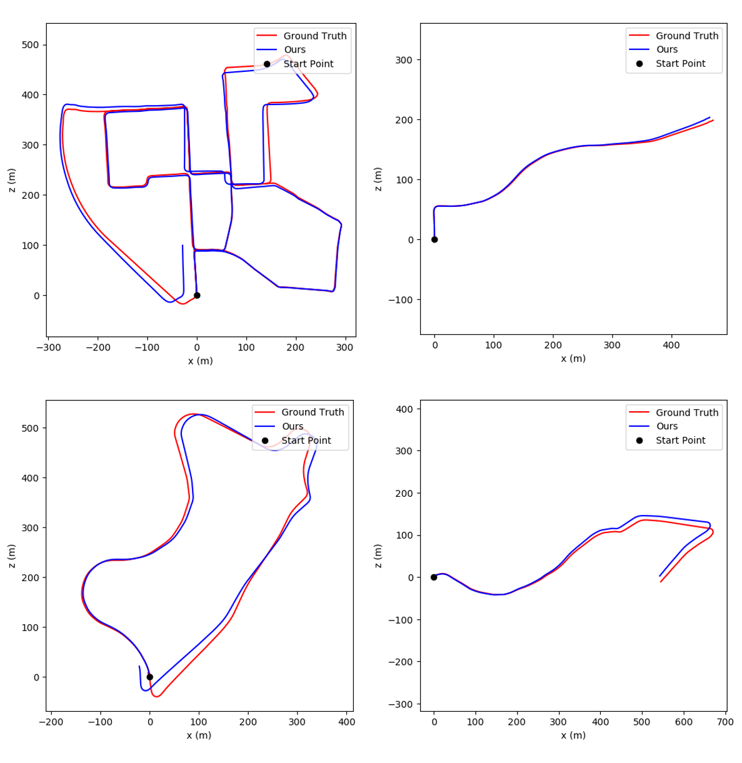
\includegraphics[width=0.4\textwidth]{Figures/train trajectory.png}
  \caption{2D estimate trajectory of our training sequences: KITTI Seq.00 (upper left), Seq.03 (upper right), Seq.09 (lower left), Seq.10 (lower right) with ground truth.}
  \label{fig:train trajectory}
\end{figure}


 Figure ~\ref{fig:train trajectory} shows our estimated 2D trajectory plots of our training sequences: KITTI sequence 00, 03, 09, and 10 with ground-truth. Figure ~\ref{fig:evaluation a} shows our estimated 2D trajectory plots of our testing sequences: KITTI sequence 07 and 08 with ground-truth. Blue line is our estimated trajectory and red line is the ground truth trajectory.  Our \lodo{} can produce accurate pose estimation with respect to ground truth. The average errors of translation and rotation with respect to path length interval of KITTI sequence 07 and 08 are shown in the Figure ~\ref{fig:evaluation b} and  ~\ref{fig:evaluation c} respectively. 



\begin{figure}[h]
\setlength{\belowcaptionskip}{-0.2cm} 
     \centering
     \begin{subfigure}[b]{0.4\textwidth}
         \centering
         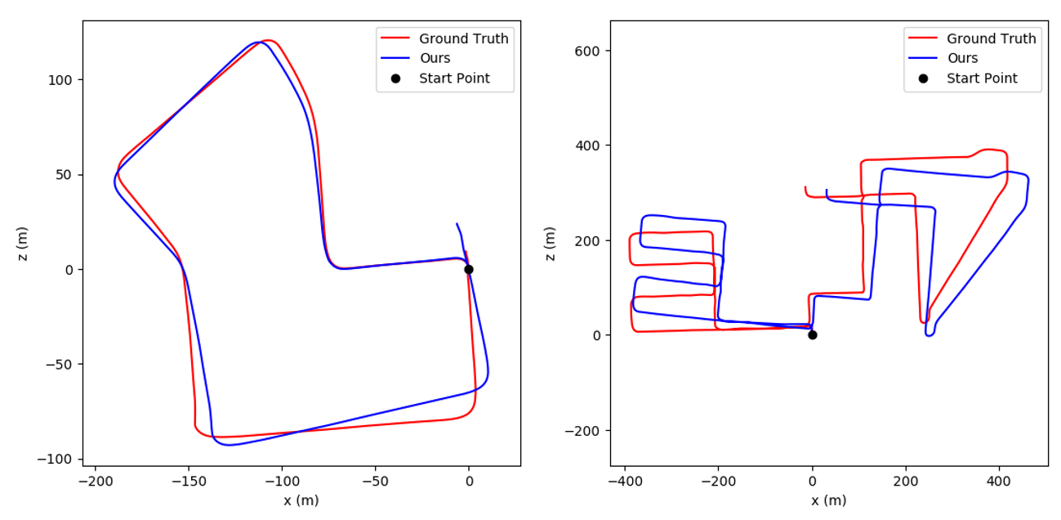
\includegraphics[width=\textwidth]{Figures/trajectory.png}
         \captionsetup{font={scriptsize}} 
         \caption{Estimated trajectory plots of KITTI Seq. 07(Left) and 08(Right) with ground truth.}
         \label{fig:evaluation a}
     \end{subfigure}

     \begin{subfigure}[b]{0.4\textwidth}
         \centering
         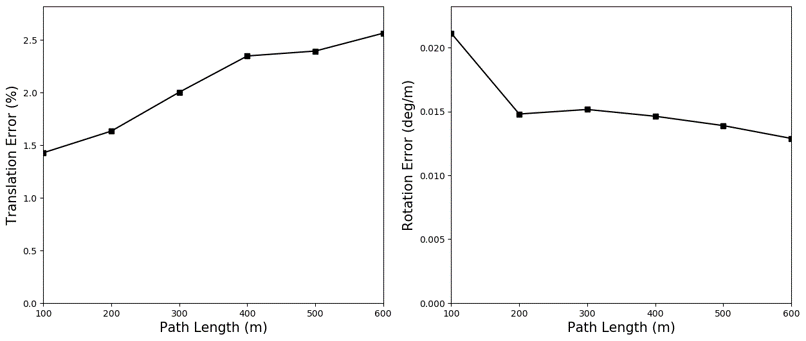
\includegraphics[width=\textwidth]{Figures/error7.png}
         \captionsetup{font={scriptsize}} 
         \caption{The average errors of translation and rotation with respect to path length interval of KITTI Seq. 07}
         \label{fig:evaluation b}
     \end{subfigure}
     
     \begin{subfigure}[b]{0.4\textwidth}
         \centering
         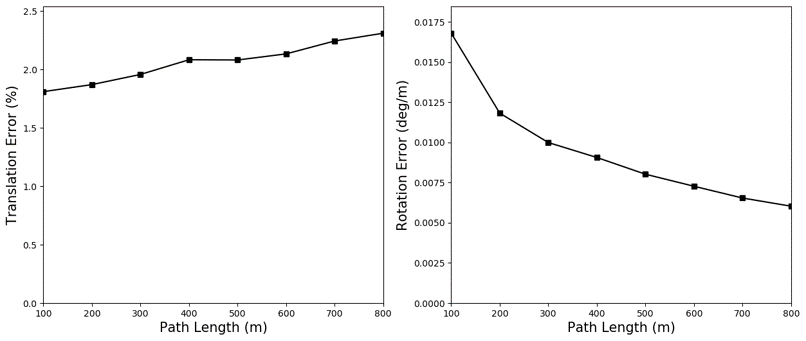
\includegraphics[width=\textwidth]{Figures/error8.png}
         \captionsetup{font={scriptsize}} 
         \caption{The average errors of translation and rotation with respect to path length interval of KITTI Seq. 08}
         \label{fig:evaluation c}
     \end{subfigure}
     
        \caption{Evaluation of our estimation on our testing set:KITTI Seq. 07 and Seq. 08}
        \label{fig:evaluation}
\end{figure}


\subsection{Ablation study}
In this section, we investigate the effects of different factors of our odometry estimation on the KITTI dataset. We change the observation parameter while others remain as default parameters to evaluate our network.

\noindent
 \textbf{Rotation augmentation in Rotation Estimation Module}

In section \ref{section:train lodo}, we clam that our rotation data augmentation procedure contribute to estimate 3-DoF relative odometry rotation information. We list the results of KITTI Seq. 07 and 08 in Table \ref{tab:ablation study rotation} with different rotation augmentation ratio. It proves that our rotation data augmentation procedure can improve our network performance and when $r$ = 0.05 achieves the best performance. 

\begin{table}
  \caption{Comparison of different combinations of the rotation augmentation ratio.}
  \scalebox{0.8}{
\begin{tabular}{c|ccccc|cl}
\hline
                        & \multicolumn{5}{c|}{{ with augmentation}}                                                                                                                                               & \multicolumn{2}{c}{{ w/o}}          \\
                      & { ratio r}                     & { 0.03} & { 0.04} & { 0.05}          & { 0.06} & \multicolumn{2}{c}{{ augmentation}} \\ \hline
                                                      & \multicolumn{1}{c|}{{ t\_rel}} & { 2.99} & { 2.48} & { \textbf{1.86}} & { 2.09} & \multicolumn{2}{c}{{ 3.77}}         \\
\multirow{-2}{*}{Seq 07}                              & \multicolumn{1}{c|}{{ r\_rel}} & { 1.79} & { 1.58} & { \textbf{1.64}} & { 1.46} & \multicolumn{2}{c}{{ 2.18}}         \\ \hline
                        & \multicolumn{1}{c|}{{ t\_rel}} & { 3.46} & { 2.09} & { \textbf{2.04}} & { 4.59} & \multicolumn{2}{c}{{ 4.33}}         \\
\multirow{-2}{*}{{ Seq 08}} & \multicolumn{1}{c|}{{ r\_rel}} & { 1.47} & { 0.98} & { \textbf{0.97}} & { 2.01} & \multicolumn{2}{c}{{ 1.80}}          \\ \hline
\end{tabular}}
\label{tab:ablation study rotation}
\end{table}

\noindent
 \textbf{Number of MKPs selected by MKPs Selection Module}

As we states in section \ref{section:Implementation detail}, we extract 1000 MKPs on consecutive spherical images. We compare the results on KITTI Seq. 07 and 08 with different numbers as shown in the Table \ref{tab:k mkp}. When choosing 100 MKPs, the network achieves the best performance. 

\begin{table}
  \caption{Comparison of top $k$ MPKs choose by MKPs selection module.}
  \scalebox{0.8}{
\begin{tabular}{c|ccccc}
\multicolumn{1}{l|}{{ }}    & { Top k}                       & { 50}   & { 100}           & { 200}  & { 300}  \\ \hline
{ }                         & \multicolumn{1}{c|}{{ t\_rel}} & { 3.70} & { \textbf{1.86}} & { 2.97} & { 4.22} \\
\multirow{-2}{*}{{ Seq 07}} & \multicolumn{1}{c|}{{ r\_rel}} & { 2.84} & { \textbf{1.64}} & { 1.89} & { 2.28} \\ \hline
{ }                         & \multicolumn{1}{c|}{{ t\_rel}} & { 3.20} & { \textbf{2.04}} & { 5.38} & { 4.09} \\
\multirow{-2}{*}{{ Seq 08}} & \multicolumn{1}{c|}{{ r\_rel}} & { 1.65} & { \textbf{0.97}} & { 2.04} & { 2.00} \\ \hline
\end{tabular}}

\label{tab:k mkp}
\end{table}

\section{Conclusions}
In this paper,we present a novel deep learning-based LiDAR odometry estimation framework named LodoNet. Within the framework we propose a new approach that extract the matched keypoint pairs(MKPs) by applying conventional image-based feature describer from projected LiDAR images. With the help of PointNet, we adopt the MKPs to estimate the movements between the LiDAR frames, which finally result in the LiDAR odometry estimation. Experiments on KITTI dataset demonstrate the effectiveness of our framework compared with existing Deep learning approaches. More over, since our framework is mainly integrated by a conventional feature describer and a light-weighed neural network, it can be easily deployed to the automated driving systems without allocating many computational resources. In our future work, we are going to explore how to further integrate the MKPs extraction and odometry estimation steps for a more accurate and efficient LiDAR odometry estimator.


% However, like many other approaches, \lodo{} can not achieve real-time LiDAR odometry estimation which means the running time must be less than 0.1s per-scan. Most of our running time is spent on the SIFT keypoint detection procedure which is computationally expensive. To speed up the running time, Fast Approximated SIFT algorithms and other time efficiency keypoint detection algorithms will be considered in the future works.
\newpage

%%
%% The next two lines define the bibliography style to be used, and
%% the bibliography file.
\bibliographystyle{ACM-Reference-Format}
\bibliography{sample-base}

\end{document}
\endinput
%%
%% End of file `sample-authordraft.tex'.
